Due to the restricted amount of memory on GPU deep learning models cannot have a high-resolution image as their input within current research. Yet this is also not obligatory: as the image contains dozens of cells within it, its processing can be limited to a crop of a smaller size. After the model has predicted fluorescence signal for each of the crops, output fluorescence images can be combined together to form a high-resolution image again. In this thesis the architecture of the model assumes an input of size $(256, 256)$ or more specifically $(None, 1, 256, 256)$, where the first dimension is responsible for the batch size and the second one states that the input is a 1-channel image. 

There are several ways of how one can split the image, the easiest approach would be to use a sliding window of size $w$. This algorithm is depicted in the Figure \ref{fig:sliding-window}. A small window starts sliding the image from the left upper to the right down corner with step size $s$ feeding the selected crops into a deep learning model. From the output of the model only a center part of such a crop is accepted to form a full fluorescence image. Border size $b$ in this case is the size of the edges of the crop that are not accepted from the predictions of the deep learning model.

Having a desired border size, in order to accepted areas to be overlaped with each other without blank spaces, one has to adjust the step size to be:
\begin{equation}
  s = w - 2 * b
\end{equation}
When step size $s$ is equal to window size $w$, there is no overlap between the windows.

\begin{figure}[H]
	\begin{center}
		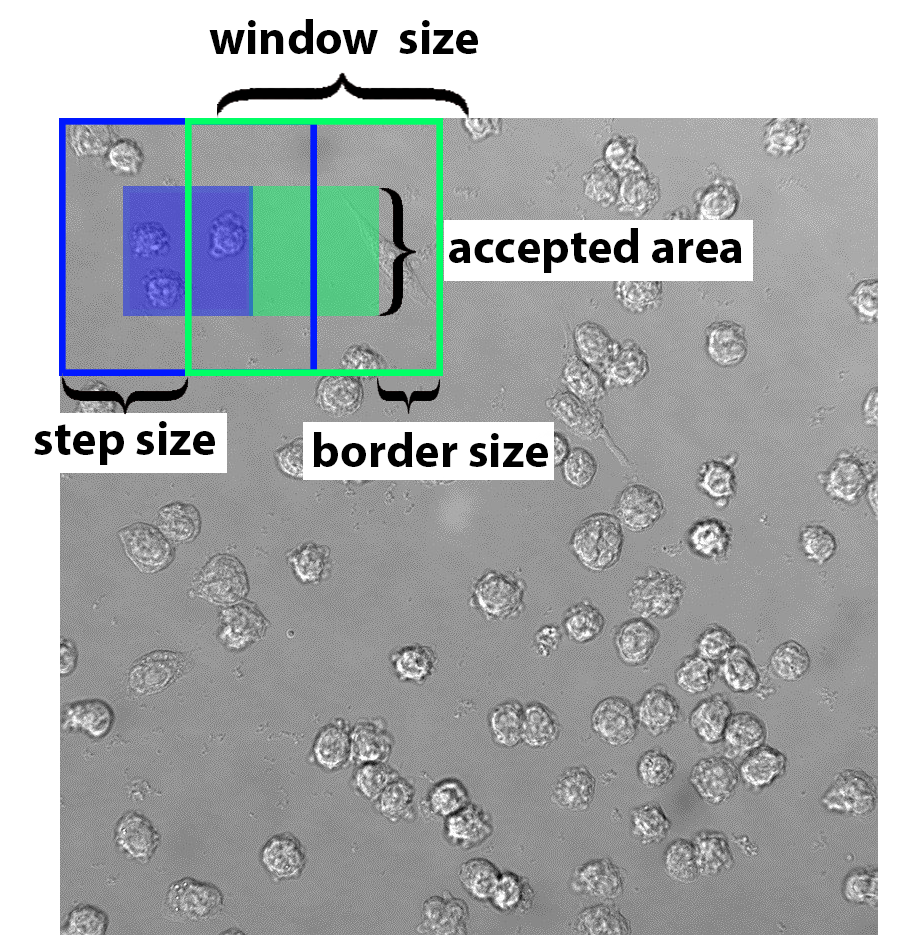
\includegraphics[width=0.3\linewidth]{bilder/sliding-window.png}
		\caption{Sliding window approach for fluorescence prediction}\label{fig:sliding-window}
	\end{center}
\end{figure}
The reason why not the full prediction is accepted to form the output hides in the following: trained models are less accurate on the borders of the crops rather than in the center. Most of the times there are cells on the borders of the crops that were sliced and therefore it might be impossible to make a good prediction for them just due to the lack of input information. Therefore the step size has to be smaller than the window size, so that the windows are overlapping and for each prediction we use only the image center and are allowed to ingore predictions on the border (see the comparison between different border sizes in the Figure \ref{fig:crops-combination}). This is dicsucced in more detail in Section [TODO reference the section]. Such approach helps to reduce the effect of the grid visible on the image composed of many small crops, which one can see in the Figure \ref{fig:crops-combination} on the left to almost non-visible borders as in the same Figure on right. This would of course take longer time in predictions, however as the speed is less crucial in comparison to the accuracy of the predictions.

\begin{figure}[htb]
	\begin{center}
		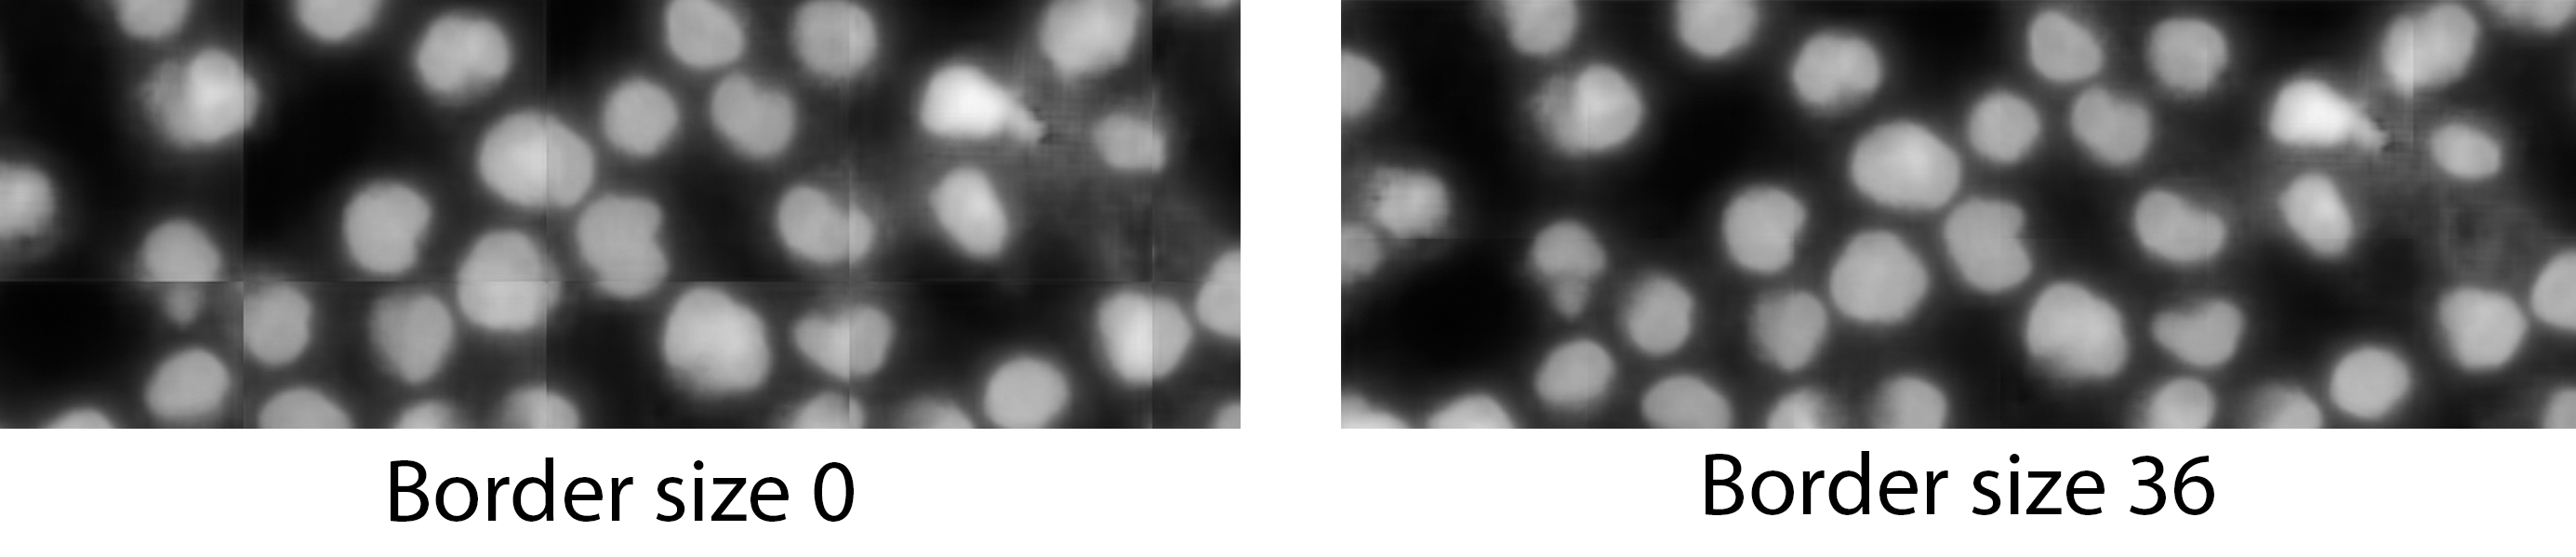
\includegraphics[width=\linewidth]{bilder/crops_combination/crops-combination.png}
		\caption{Difference of overlap between predictions on the resulting image}\label{fig:crops-combination}
	\end{center}
\end{figure}